\FloatBarrier
\subsection{RLS identification with gradual parameter change}
This section uses the Simulink model shown in \autoref{fig:RLSISGCSimulinModel}. The system's $a_2$ and $a_3$ parameters are gradually changed, as detailed in the MATLAB code provided in \autoref{code:RLSISGCGradualChange}. Specifically, $a_2$ is reduced to $30\%$ of its initial value between samples $50$ and $101$, and  $a_3$ is similarly reduced between samples $200$ and $251$. The system features a white noise input with a variance of $2$, and white noise is also present on the output.

\begin{code}
	\begin{matlabcode}{firstnumber = 12}
	%% Gradually change parameters
	a2 = ones(signal_length);a2=a2(1:end,1:2);
	a3 = ones(signal_length);a3=a3(1:end,1:2);a3(:,2)=1/6*a3(1:end,2);
	
	% Calculate the step size for a linear change
	%final_value-initial_value/sample_period
	step_size_a2 = (0.3 - 1) / 50;
	step_size_a3 = ((0.3*(1/6)) - 1/6) / 50;
	
	for n=1:length(a2(1:end,1))
	a2(n,1) = 0.3*n;
	a3(n,1) = 0.3*n;
	end
	
	% change a2 form 50 to 101
	for n=50:101
	a2(n,2) = a2(n,2)+step_size_a2*(n-50);
	end
	a2(101:end,2) = a2(101,2);
	
	% change a3 form 200 to 251
	for n=200:251
	a3(n,2) = a3(n,2)+step_size_a3*(n-200);
	end
	a3(251:end,2) = a3(251,2);
	\end{matlabcode}
	\captionof{listing}{Gradual change of parameters}
	\label{code:RLSISGCGradualChange}
\end{code}



\begin{figure}
	\centering
	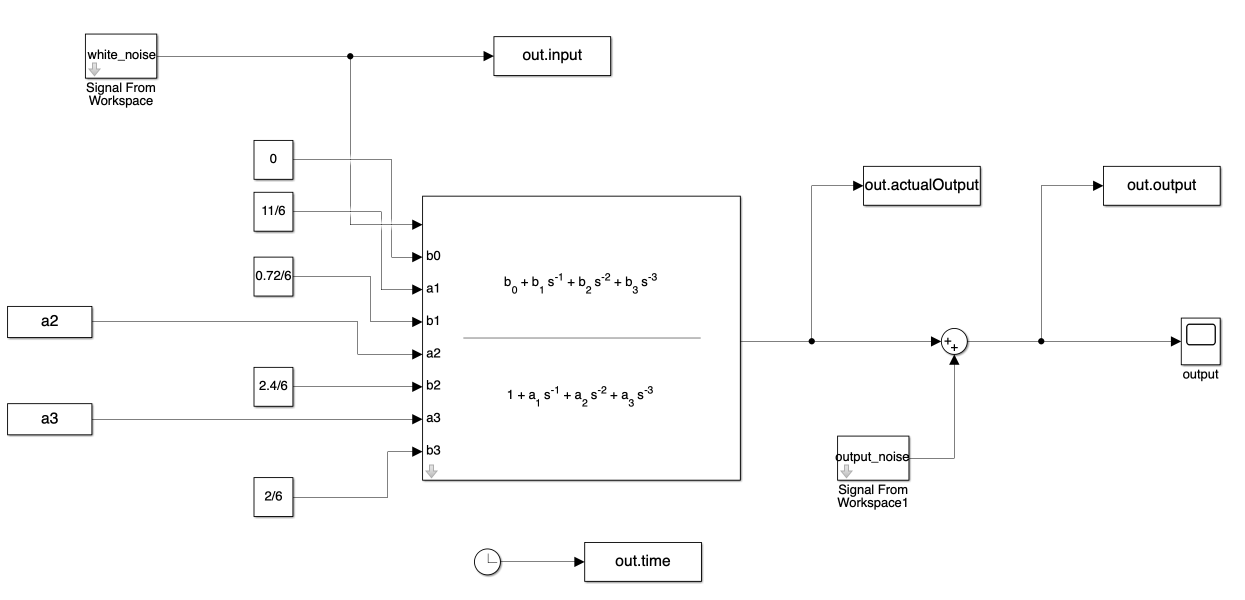
\includegraphics[totalheight=8cm]{images/RLSISGCSimulinkModel.png}
	\caption{RLS system output with gradual change}
	\label{fig:RLSISGCSimulinModel}
\end{figure}

\autoref{fig:RLSISGCOutput} displays the system's output and associated error calculations. \autoref{fig:RLSISGCParams} illustrates the parameter evaluation throughout the program's execution. The final identified transfer function is shown in \autoref{eq:RLSISGCTransferFunction}. To improve parameter estimation, we incorporated a forgetting factor.

\begin{figure}
	\centering
	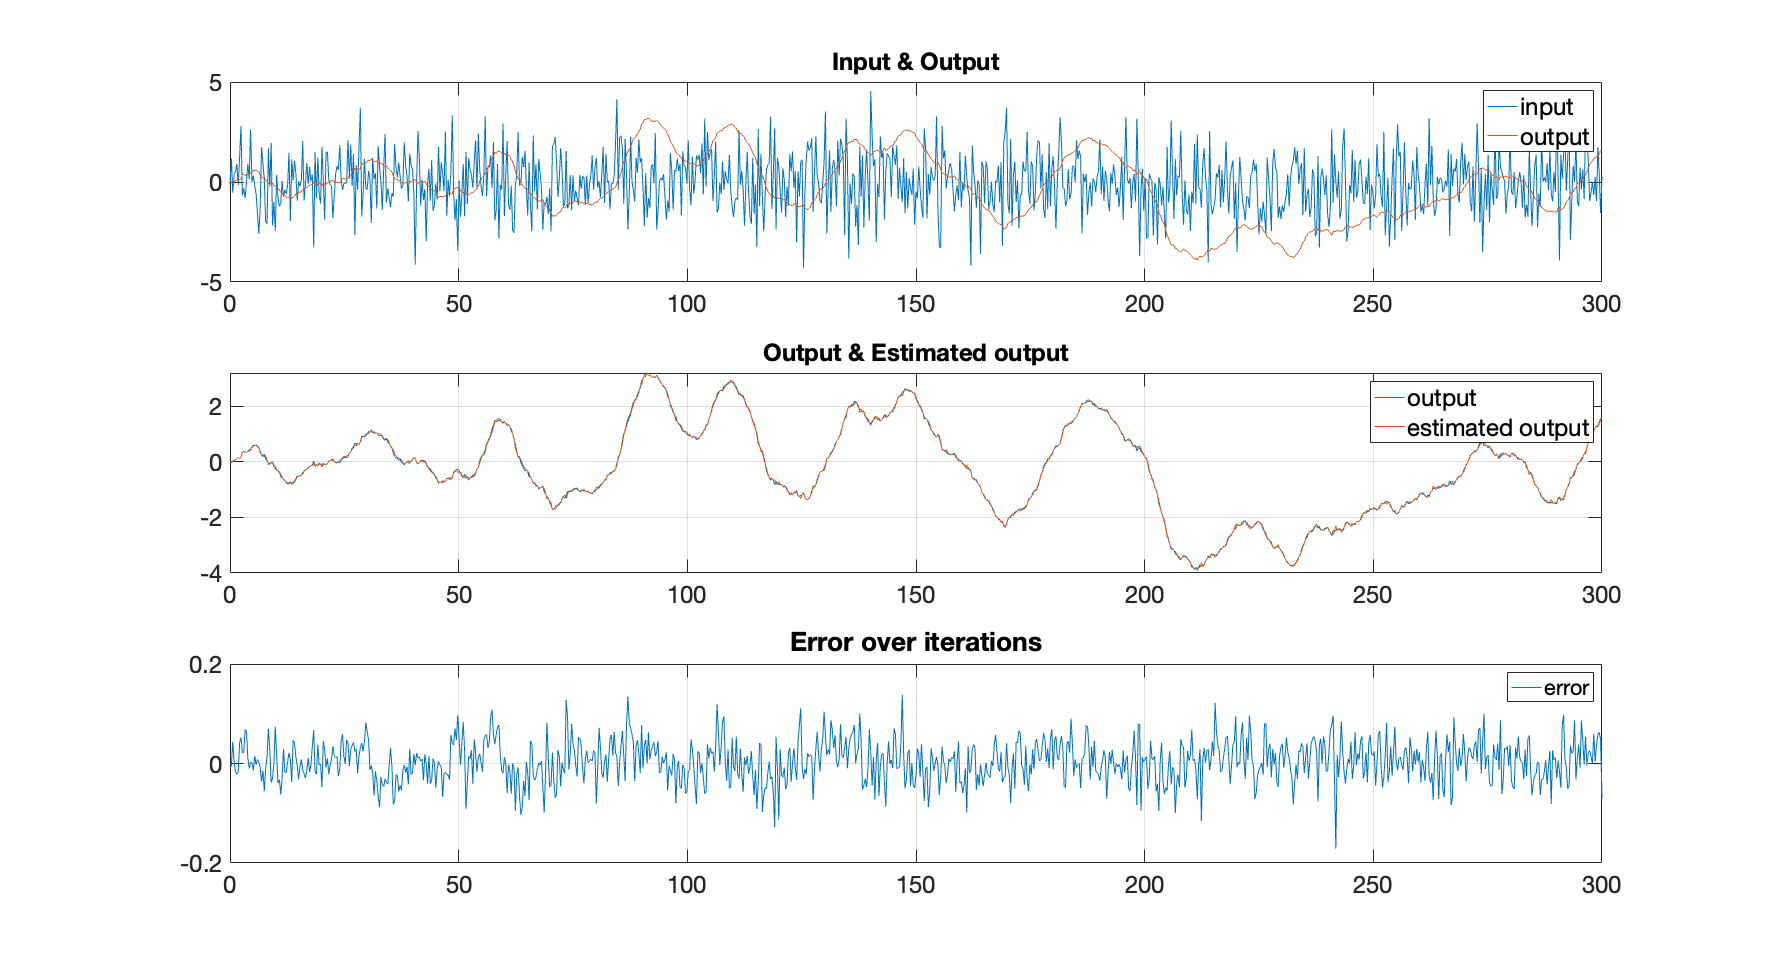
\includegraphics[totalheight=8cm]{images/RLSISGCOutput.png}
	\caption{RLS system output with gradual change}
	\label{fig:RLSISGCOutput}
\end{figure}
\begin{figure}
	\centering
	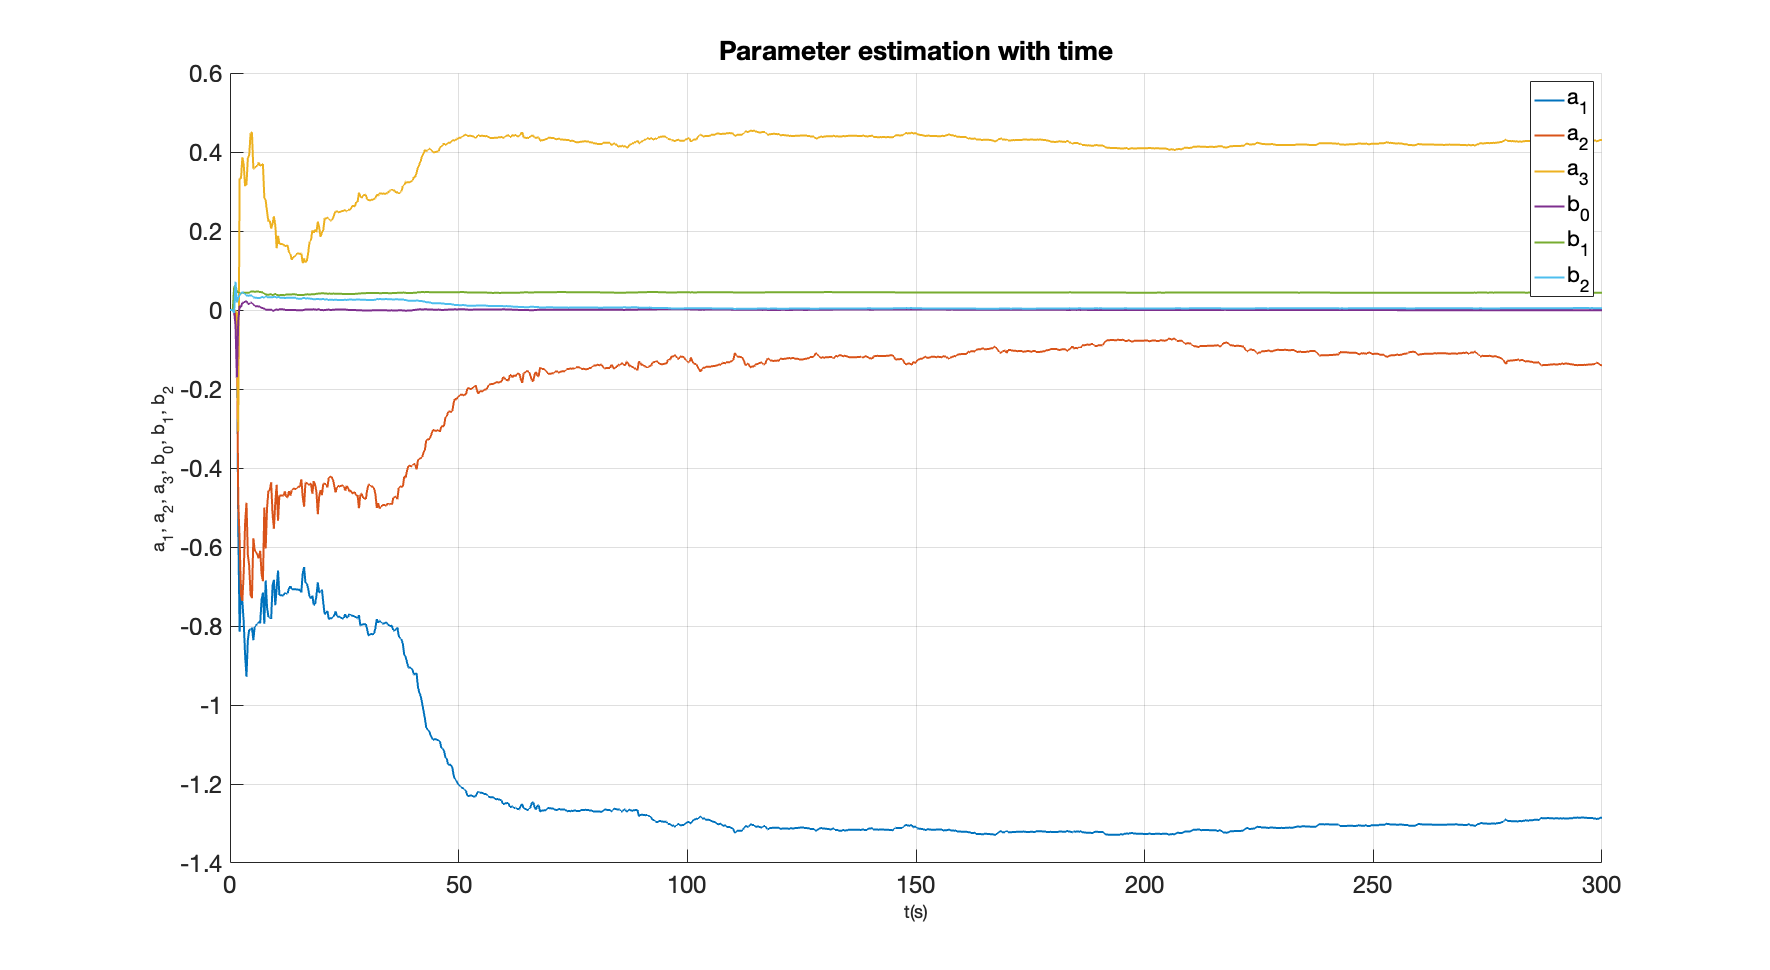
\includegraphics[totalheight=8cm]{images/RLSISGCParams.png}
	\caption{RLS system parameters with gradual change}
	\label{fig:RLSISGCParams}
\end{figure}
\begin{equation}
	G(z) =	\frac{0.0006954 z^2 + 0.04372 z + 0.004116}{z^3 - 1.297 z^2 - 0.1275 z + 0.4299}
	\label{eq:RLSISGCTransferFunction}
\end{equation}

\autoref{fig:RLSISGCFixedOutput} shows the improved identification of the system. \autoref{fig:RLSISGCFixedOutputParams} shows the improved parameter estimation for the given system. The resulted transfer function is presented at \autoref{eq:RLSISGCFixedTransferFunction}. 

\begin{figure}
	\centering
	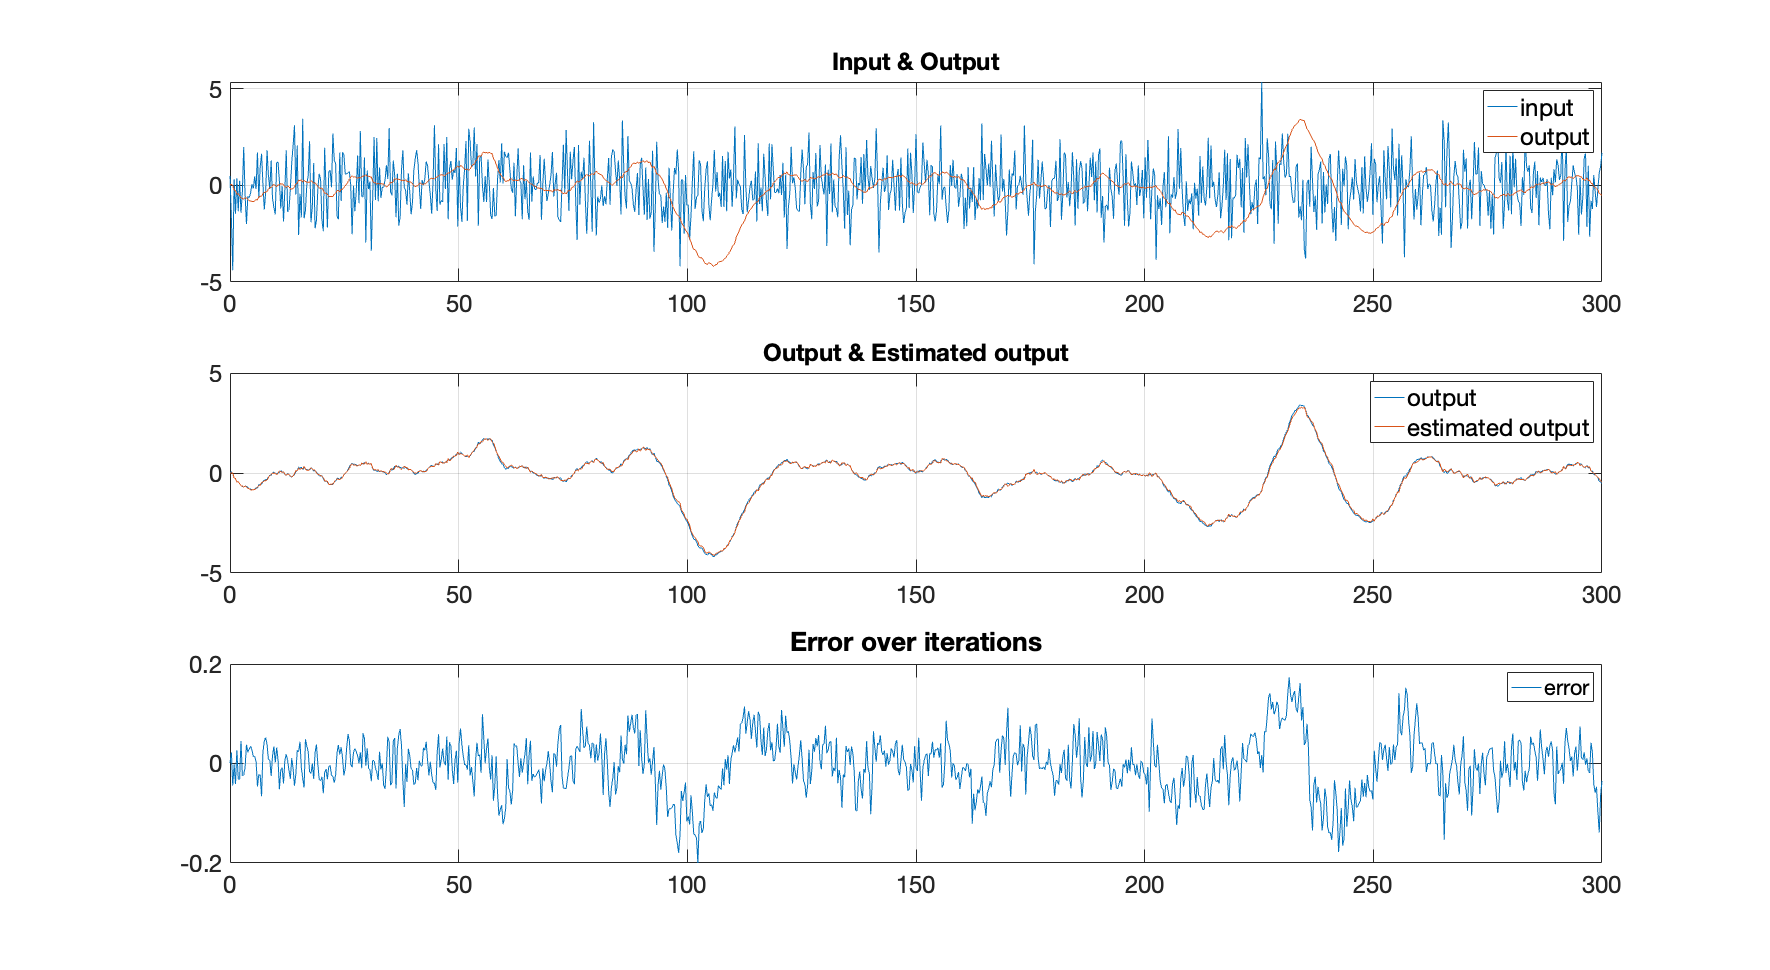
\includegraphics[totalheight=8cm]{images/RLSISGCFixedOutput.png}
	\caption{Improved RLS system output with gradual change}
	\label{fig:RLSISGCFixedOutput}
\end{figure}
\begin{figure}
	\centering
	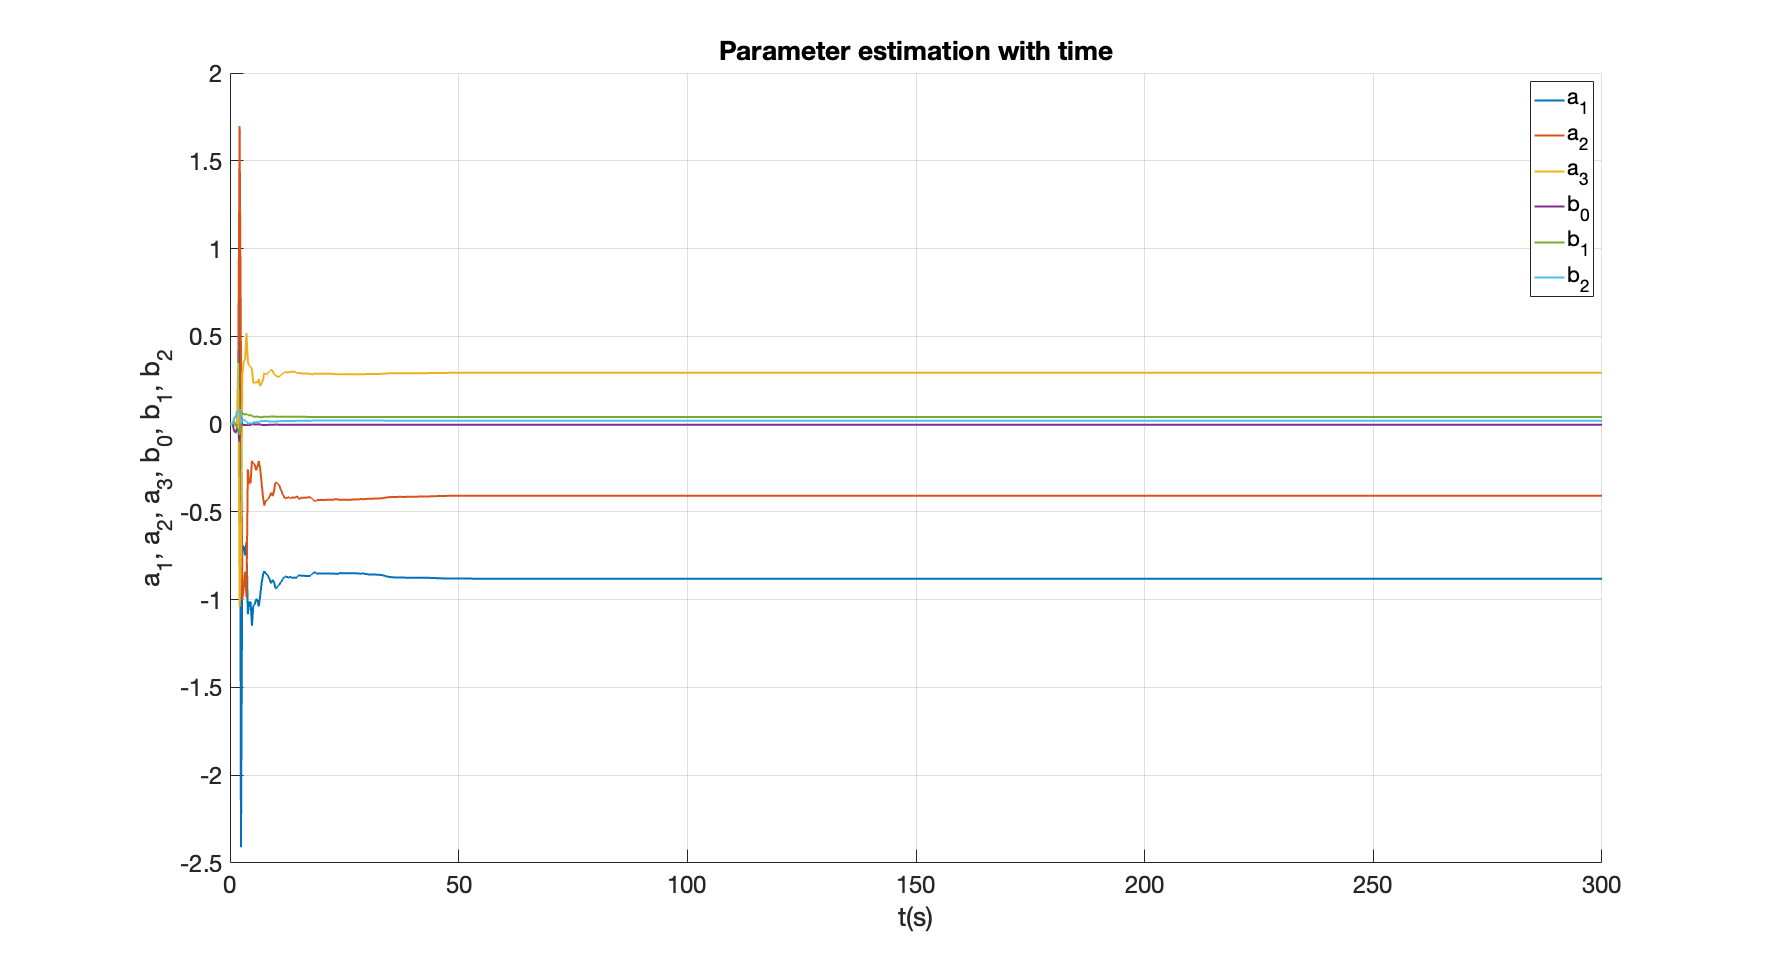
\includegraphics[totalheight=8cm]{images/RLSISGCFixedParams.png}
	\caption{Improved RLS system parameters with gradual change}
	\label{fig:RLSISGCFixedOutputParams}
\end{figure}
\begin{equation}
	G(z) =	\frac{-0.001267 z^2 + 0.04973 z + 0.01321}{z^3 - 0.9687 z^2 - 0.2906 z + 0.2769}
	\label{eq:RLSISGCFixedTransferFunction}
\end{equation}

The Simulink model can be accessed at \hspace{-1ex}\lstinline| assignment1/part2/2_6/RLS2_6_NS.slx|.
Matlab code for system is at \hspace{-1ex}\lstinline| assignment1/part2/2_6/RLS2_6_noise.m| and for improved system identification is at \hspace{-1ex}\lstinline| assignment1/part2/2_6/RLS2_6_fix.m|.